\section{User-centered Design}


\textbf{Design Intention vs User Needs}

\textit{Prototyping as an interative process}

\begin{center}
	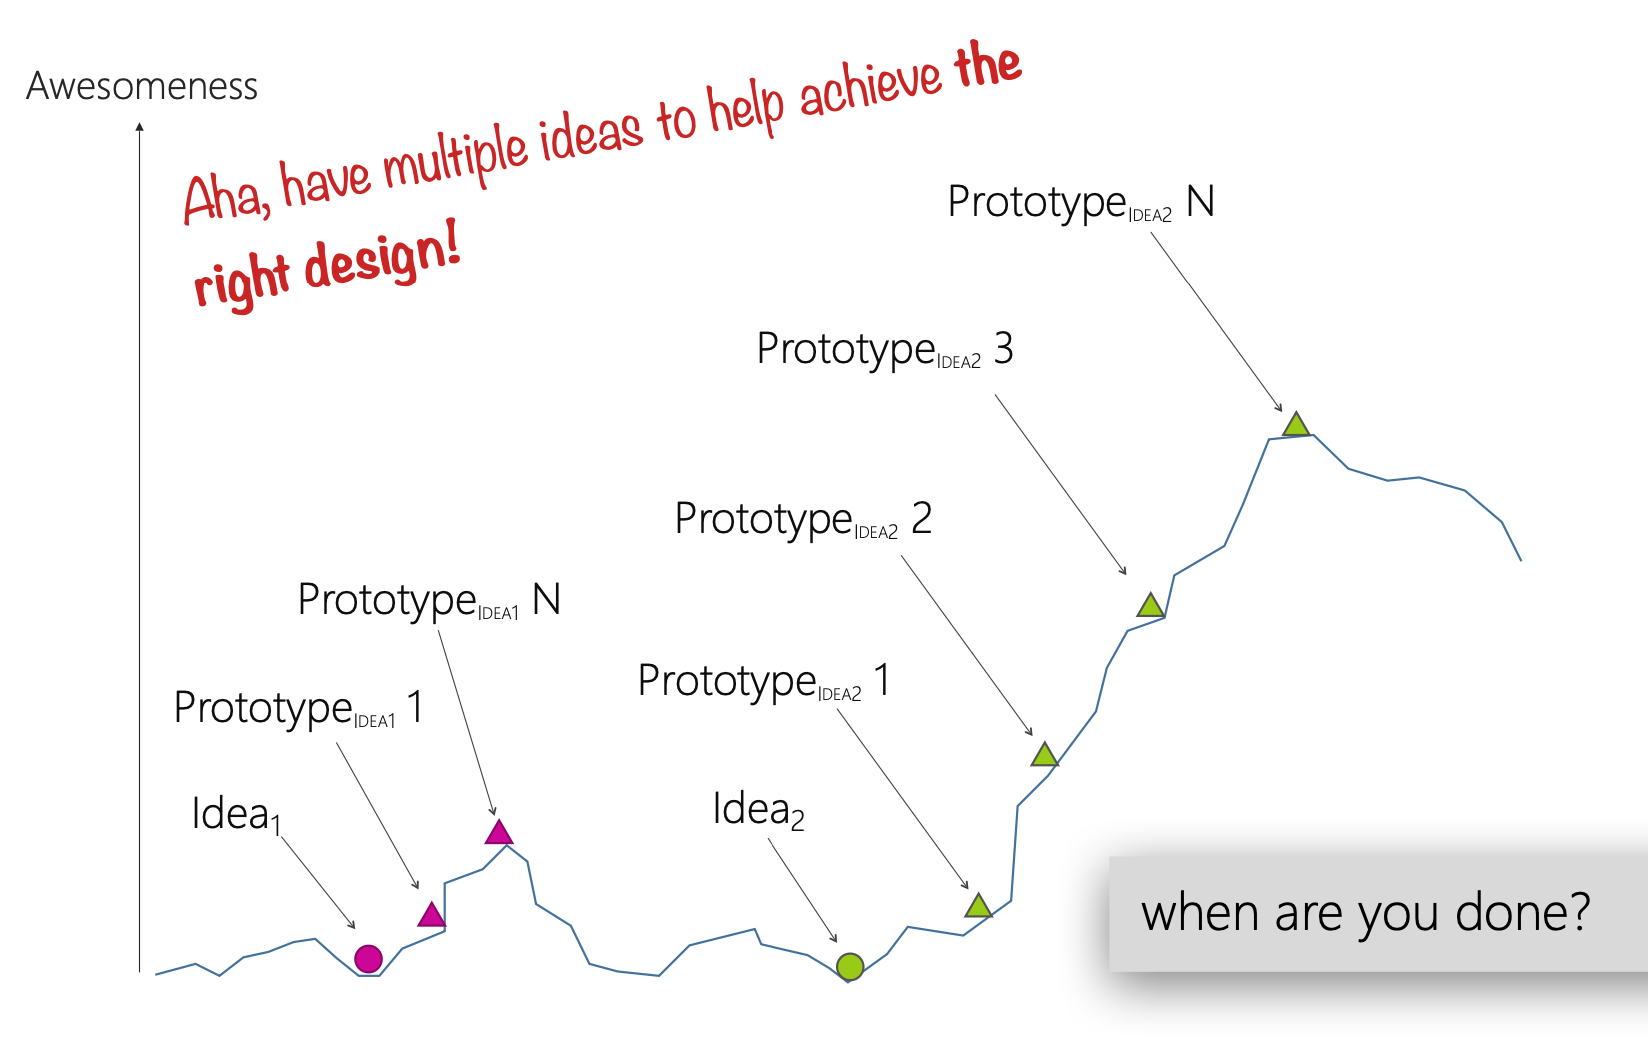
\includegraphics[width=\linewidth]{iterative_process.png}
\end{center}
Does the design work properly in the context of use? If not fix the problems and carry out more tests. \medskip

\textbf{Early focus on users and tasks:} \smallskip

Cognitive, behavioral, anthropomorphic AND attitudinal characteristics. \medskip

\textbf{Empirical Measurement:} \smallskip

Observe user's reactions and performance in scenarios, manuals simulations and prototypes, record and analyze. \medskip

\textbf{Root-Cause Analysis} \smallskip

Problems need to be discovered (find the right problem to solve, not any problem to solve) and find the right solution to it. \medskip

\textbf{Need finding} \smallskip

Users rarely know what they want. They cannot imagine what is possible. Instead look at tasks, context: 

\begin{multicols}{2}
    \begin{itemize}[itemsep=-5pt, topsep=-20pt, leftmargin=*]
	\item What information needed?
	\item Identify collaborators
	\item Why is task achieved the way it is?
	\item Identify tasks in existing behavior
	\item Identify tasks in future scenarios
	\end{itemize}
\end{multicols}

We ourselves are not representative of the typical user. To learn about customers we conduct interviews, self-reports and logging/analytics.
We also observe users performing tasks and understand their cognition. \medskip

\textbf{Understanding the User} \smallskip

Active observation is not knowing yet what we are looking for. 

\begin{multicols}{2}
    \begin{itemize}[itemsep=-5pt, topsep=0pt, leftmargin=*]
	\item Immerse
	\item Observe
	\item Engage

	\end{itemize}
\end{multicols}


\begin{center}
	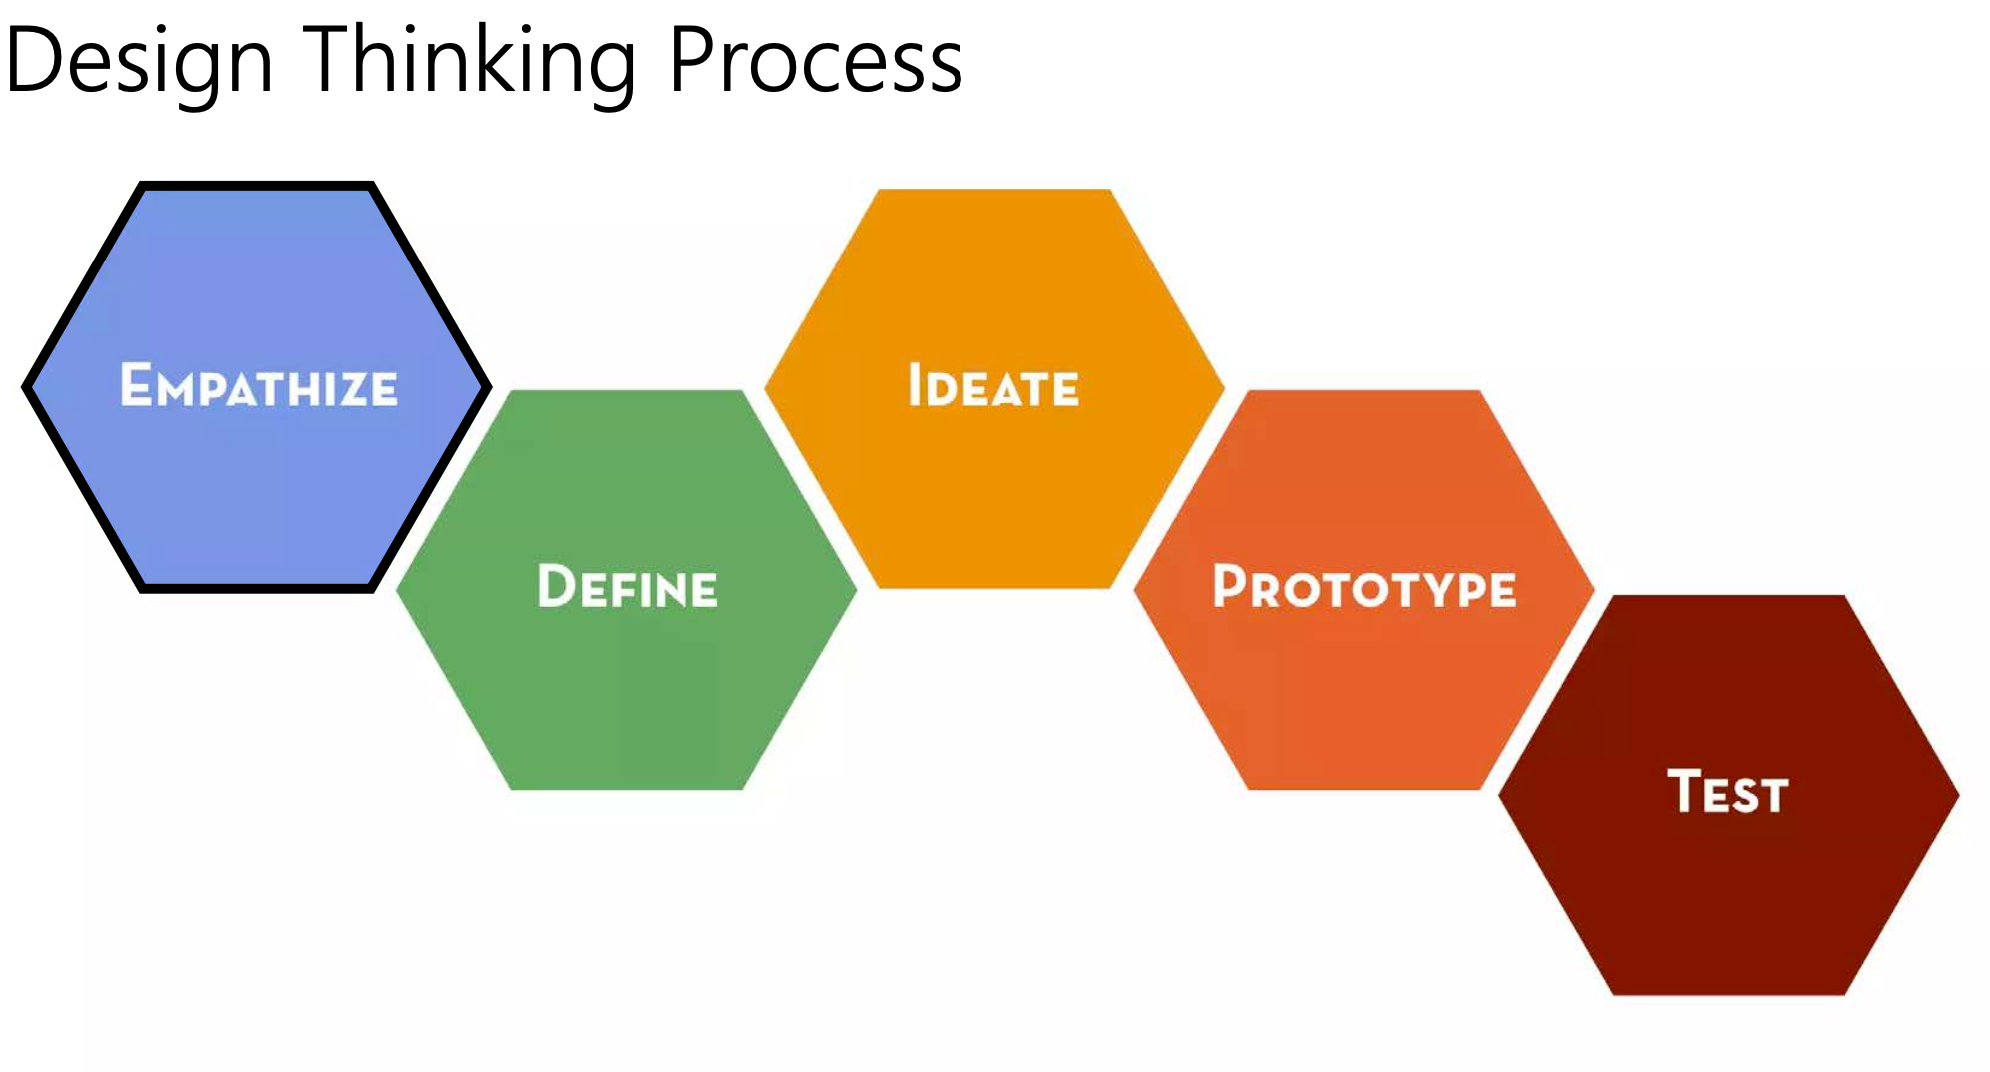
\includegraphics[width=\linewidth]{design_thinking_process.png}
\end{center}


\textbf{Goals of Need finding}


\begin{itemize}[itemsep=-5pt, topsep=3pt, leftmargin=*]
	\item Distill useful and actionable insights
	\item Make meaning from needfinding data
	\item reframe problem to guide solution search
\end{itemize}

\medskip

We start with closed ended questions and move to open ended questions: "What's and why's of feelings". Engage people in their environment.
The goal is to find inspiring users, that surprise us and bring us to game-changing ideas. \medskip

\textbf{Needs vs. features vs. requirements}

Requirements are goals that the system needs to accomplish. Solutions fulfill requirements. What does the user want to accomplish and how is he doing it?
What would they like to be doing? What are they currently disliking? For what is the system usable and what tasks will it support? Answering these questions will make the system more usable. \medskip

There are tons of methods to needfinding such as: 

\begin{multicols}{2}
    \begin{itemize}[itemsep=-5pt, topsep=-20pt, leftmargin=*]
	\item Task Analysis
	\item Interviews
	\item Affinity Diagrams
	\item Cognitive Walkthrough
	\item Questionnnaires
	\item Focus Groups
	\item Diary Studies
	\item "Speed dating"
	\item etc.
	\end{itemize}
\end{multicols}

\textbf{Interview}

Interviewee speaks 90 percent of time and stays on topic. We choose participants to be representative target users, either current or potential future users. We like both experts and typical users. Try to provide an explanation into how users make sense to themselves. \medskip

\textbf{Common pitfalls in interviews} \smallskip

Suggesting answers. Hypthetical questions. \medskip

\textbf{Diary Study} \smallskip

Ask people to record events as they happen. 
User diary studies for rare events, easily forgotton events and events where the actual frequency is important. 
Problems with diary studies is that the simple tracking of their behaviors will change their behaviors. \medskip

\textbf{Retrospective Survey} \smallskip

Ask about things that have happened in the past. Use this for critical events (well remembered), recent and memorable events, rare events that had a big impact an are memorable. Do not use them for hard to remember events.\medskip

\textbf{Artifact Analysis} \smallskip

Look at things people leave around to understand a problem they might have. Use this for physical spaces (physical artifacts from workflows), tasks involving artifacts and interactions generating artifacts (emails, social media posts etc.).
Only use if there are in fact artifacts and there is no faster way to learn information. \medskip

\textbf{Contextual Inquiry} \smallskip

Ethnographics or participatory design, combining aspects of other methods. Interviewing, observing in the context of work. Goal is to discover real requirements of the work.
Interview people while they are working and gather real artifacts. User decides the tasks, but you decide the focus. \medskip

\columnbreak

\textbf{Key Differences}


\begin{center}
	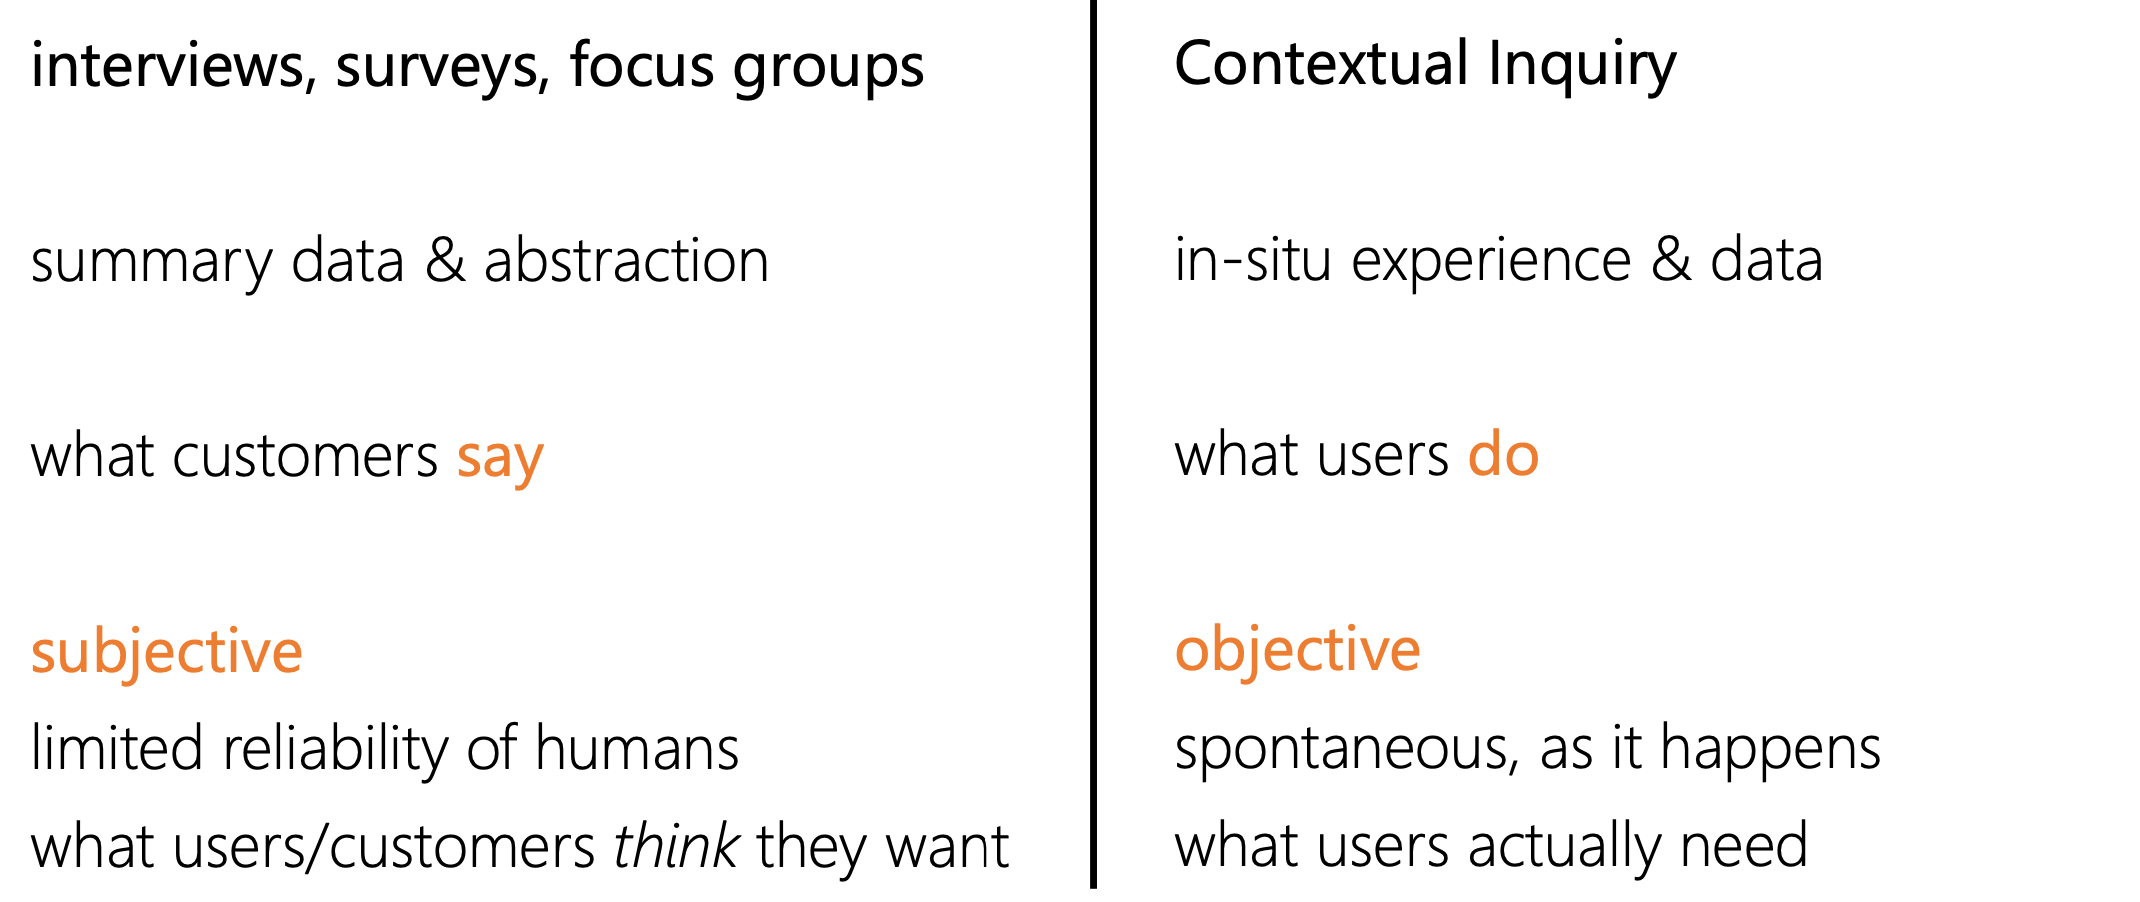
\includegraphics[width=\linewidth]{differences.png}
\end{center}

\textbf{Result of Need-Finding} \smallskip

We know what works and what does not yet exist. Problems and incomplete parts in process. So we have a long list of problems. 


\begin{center}
	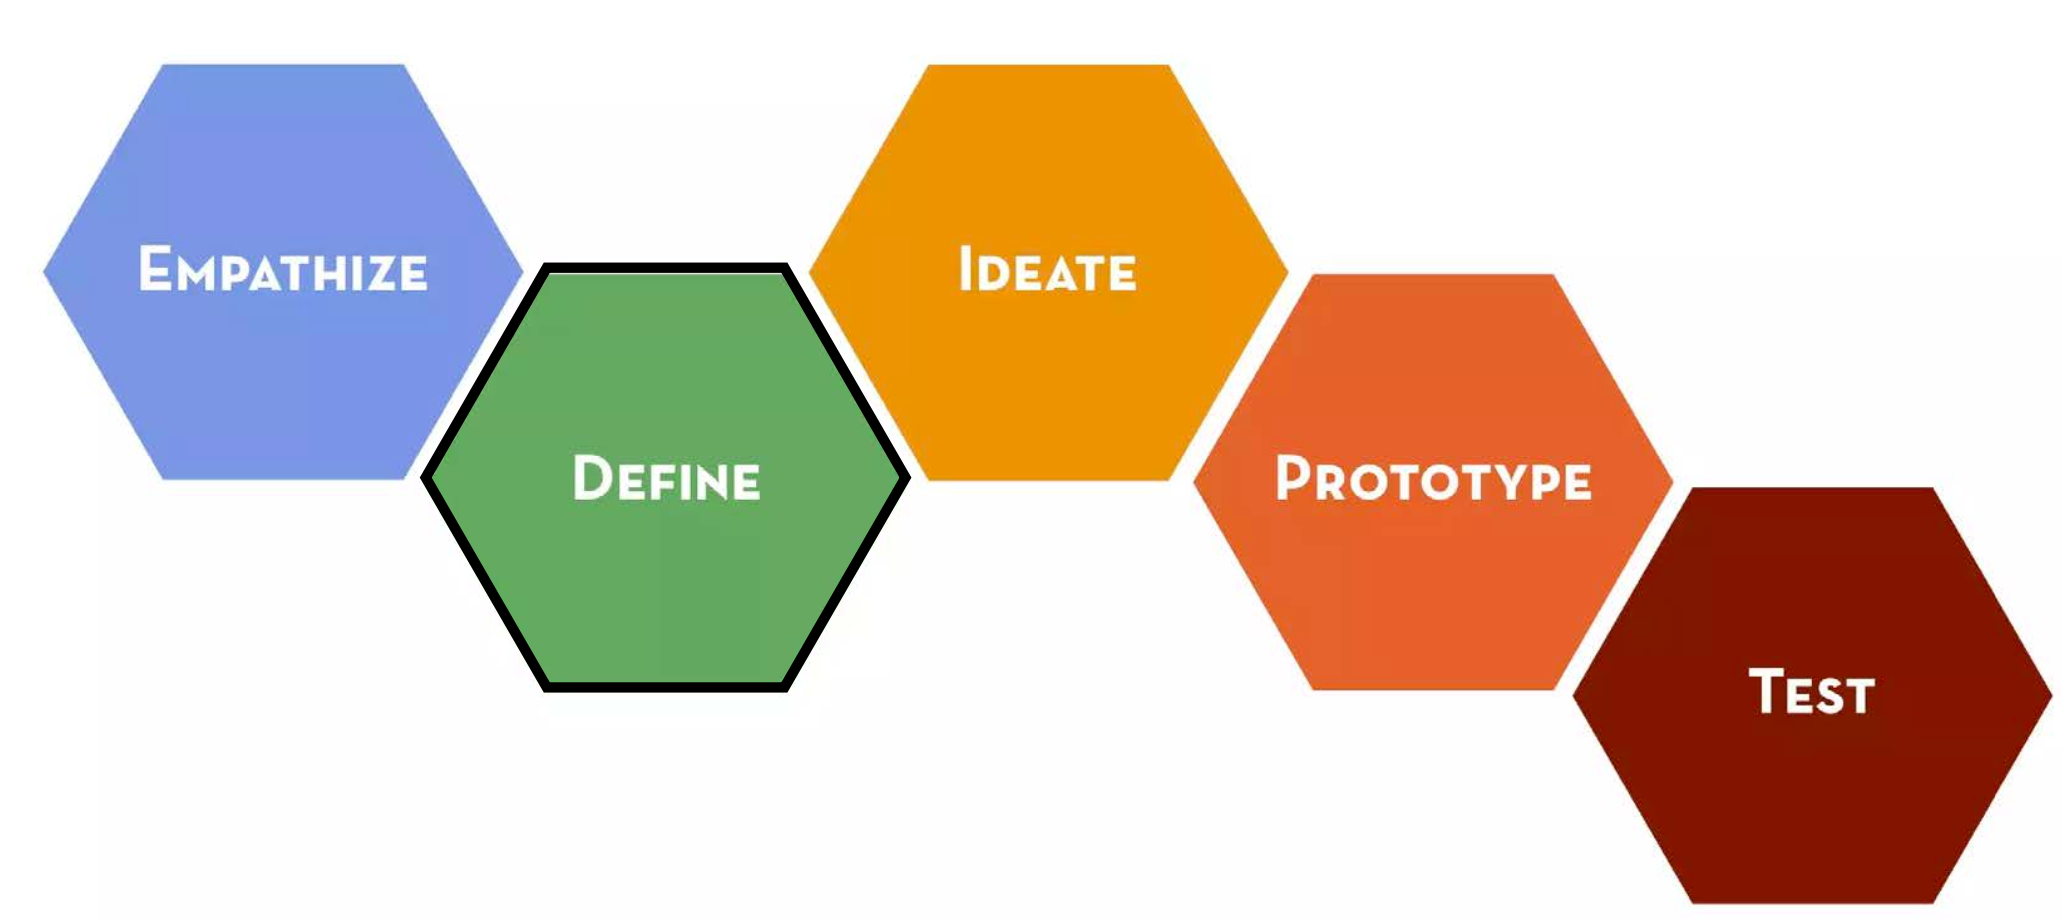
\includegraphics[width=\linewidth]{define.png}
\end{center}

\textbf{Define} \smallskip

This part is more a focussing part and not flaring. Figure out what is important from collected data. Group info and find relations. \medskip

\textbf{Affinity Diagrams} \smallskip

Data with affinity to each other are grouped together to form category. Groups are given labels, can be one or more categories in the end. 
Identify user, need and insight. Combined to create point of view. 
Good point of view insires the team, frames the problem in a focussed way. Empowers to make decisions and fuels brainstorming by suggesting "how might we" statements. \medskip

\textbf{The elastic user} \smallskip

The elastic user can mean everyone and also noone. Vague and unfocused, lack of specifics makes it easy to rationalize any design. \medskip

\textbf{Personas} \smallskip

Personas are precisely described. Act as stand-in for real users. Guide design decision. Fictitious but based on knowledge of real users. Informed from observations.
Personas are not elastic, don't make them fit the prototype. 

\begin{center}
	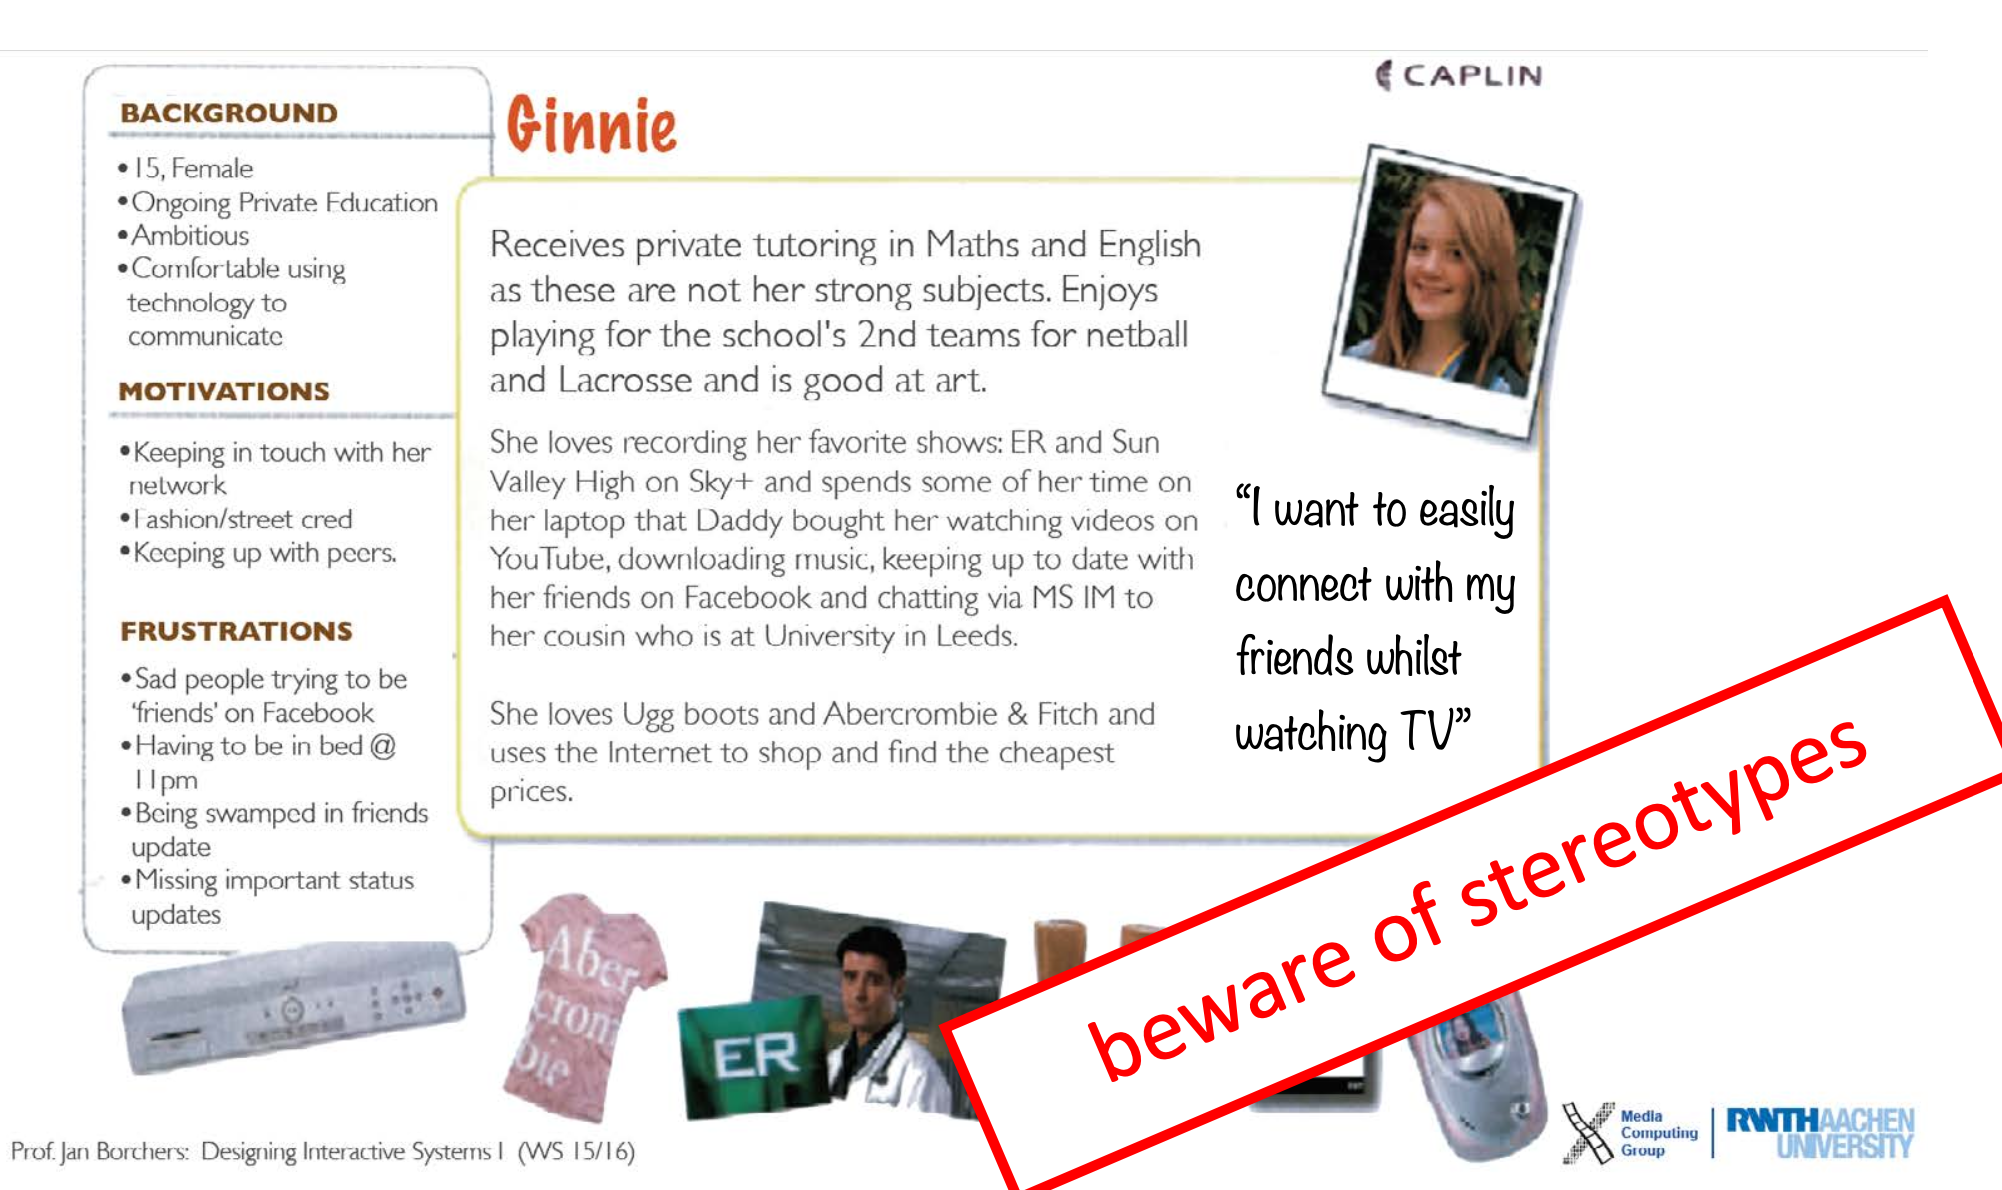
\includegraphics[width=\linewidth]{persona.png}
\end{center}

\begin{center}
	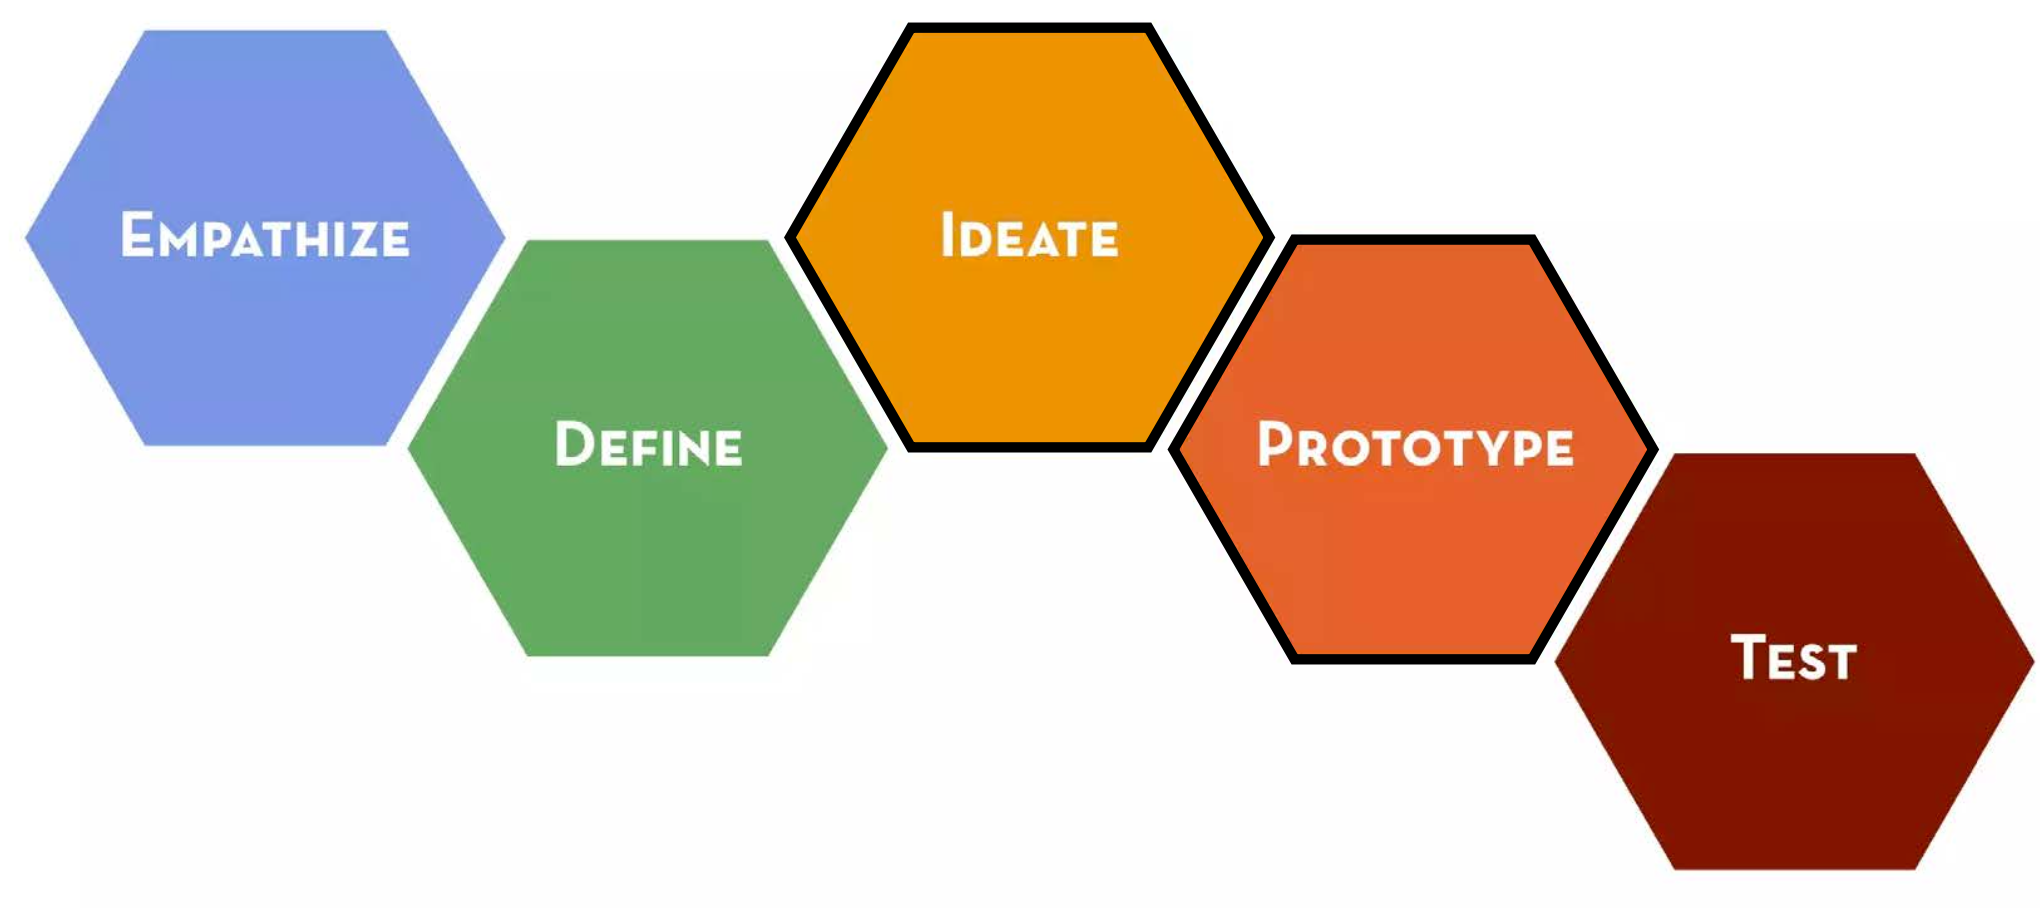
\includegraphics[width=\linewidth]{ideate.png}
\end{center}

\textbf{Ideate} \smallskip

Flaring process here, not focussing anymore. \medskip

\textbf{Ideation techniques}

\begin{multicols}{2}
    \begin{itemize}[itemsep=-5pt, topsep=-20pt, leftmargin=*]
	\item brainstorming
	\item mind-mapping
	\item storyboarding
	\item sketching
	\item low-fi prototyping
	\end{itemize}
\end{multicols}

\columnbreak
